\section{Introduction to Probability}
\subsection{Zufallsvariable}
Eine Zufallsvariable X (oder anderer Grossbuchstabe) ist eine Variable, die einen numerischen Wert x (Kleinbuchstabe) zuordnet, welche aus einem Zufallsexperiment kommt.\\

Es gibt zwei Arten von Zufallsvariablen:
\begin{itemize}
\item \textbf{Diskret}: X nimmt einen fixen Wert an aus einer fix definierten Zahlenmenge: {1.56, 2.93, 4, 6, 8}
\item \textbf{Stetig}: X nimmt einen Wert aus einem unzählbaren bereich. Z.B alle Zahlen im Intervall (2, 7)
\end{itemize}

Vergleich mit anderen Variablen:
\begin{itemize}
\item \textbf{Algebra}: In einer expression ‘x+2=10’ ist eine variable ein wert, wo eine Gleichung in einen richtigen Ausdruck bringt.
\item \textbf{Programmierung}: Hier ist einer Variable eine Zuweisung. Die Variable kann ihren Wert mit jeder Neuzuweisung ändern.
\end{itemize}

Vor der Ausführung eines Zufallsexperiments ist das beste, das wir machen können eine Liste mit allen möglichen Werten mit den zugehörigen Wahrscheinlichkeiten.

Beispiel mit Würfel:

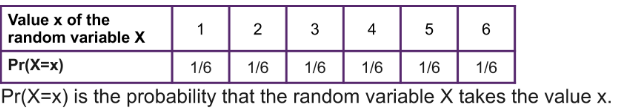
\includegraphics[width=\linewidth]{img/dice.png}

\subsection{Wahrscheinlichkeitsfunktion (Probability Mass Function PMF)}
Die Wahrscheinlichkeitsfunktion einer diskreten Variable ist eine Funktion, welche die Warscheinlichkeit angibt für jeden möglichen x-Wert. Als Beispiel kann man das obige Beispiel mit dem Würfel anschauen. Sie definiert auch eine Wahrscheinlichkeitsverteilung (Probability Distribution). Wird meist als Synonym verwendet.
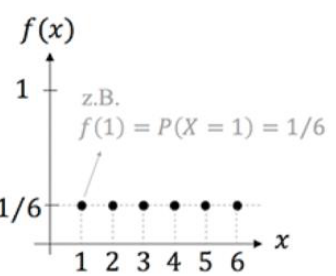
\includegraphics[width=\linewidth]{img/pmf.png}

\subsection{Zwei Zufallsvariablen}
Man kann auch zwei Zufallsvariablen gleichzeitig ansehen. Z.B X ist Augenzahl von Würfel 1 und Y ist Augenzahl von Würfel 2. Dann kann das Zufallsexperiment sein, dass man zwei Würfel wirft, was 36 Möglichkeiten gibt. Jede Möglichkeit ist gleich wahrscheinlich.
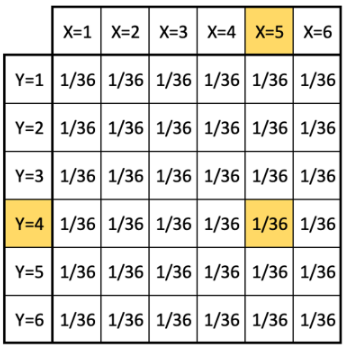
\includegraphics[width=\linewidth]{img/zwei_zufallsvariablen.png}

\subsection{Zusammengesetzte Warscheinlichkeit (Joint Probability Mass Function)}
Die zusammengesetzte Wahrscheinlichkeit oben beschreibt z.B die Warscheinlichkeit das Augenzahl Y=4 und Augenzahl X=5 ist. Diese beträgt 1/36. Man schreibt dies auch Pr(X=5, Y=4) = 1/36 oder P(5,4) =  1/36

\textcolor{myblue}{Unabhängig:}
Im oben genannten Beispiel sind die beiden Zufallsvariablen unabhängig. Ein Würfelwurf beinflusst das andere Exgebnis nicht. Also gilt folgende Formel:\\
P(X, Y) = P(X) * P(Y)     (wenn X und Y unabhängig sind)\\
P(X, Y, Z) = P(X) * P(Y) * P(Z)    (wenn X, Y und Z unabhängig sind)

\textcolor{myblue}{Bedingte Warscheinlichkeit (Correlated Random Variable):}
Doch unabhängig ist eher die Ausnahme als die Regel. Meist sind die Variablen Abhängig voneinander. \\
Joint Probability P(X,Y) und Conditional Probability P(X|Y) (X wenn Y) sind wie folgt miteinander verknüpft:\\
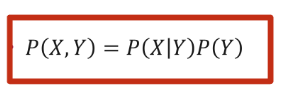
\includegraphics[width=\linewidth]{img/correlated_random_variable.png}
\textcolor{myblue}{Satz von Bayes:}\\
Ebenso gilt der Satz von Bayes:\\
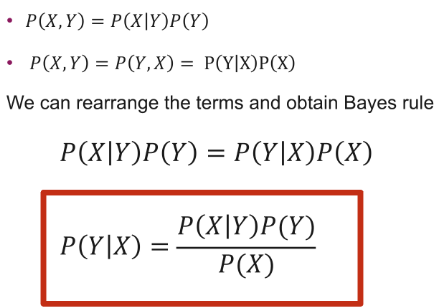
\includegraphics[width=\linewidth]{img/bayes.png}
TODO include examples